%Version 3.1 December 2024
% See section 11 of the User Manual for version history
%
%%%%%%%%%%%%%%%%%%%%%%%%%%%%%%%%%%%%%%%%%%%%%%%%%%%%%%%%%%%%%%%%%%%%%%
%%                                                                 %%
%% Please do not use \input{...} to include other tex files.       %%
%% Submit your LaTeX manuscript as one .tex document.              %%
%%                                                                 %%
%% All additional figures and files should be attached             %%
%% separately and not embedded in the \TeX\ document itself.       %%
%%                                                                 %%
%%%%%%%%%%%%%%%%%%%%%%%%%%%%%%%%%%%%%%%%%%%%%%%%%%%%%%%%%%%%%%%%%%%%%

%%\documentclass[referee,sn-basic]{sn-jnl}% referee option is meant for double line spacing

%%=======================================================%%
%% to print line numbers in the margin use lineno option %%
%%=======================================================%%

%%\documentclass[lineno,pdflatex,sn-basic]{sn-jnl}% Basic Springer Nature Reference Style/Chemistry Reference Style

%%=========================================================================================%%
%% the documentclass is set to pdflatex as default. You can delete it if not appropriate.  %%
%%=========================================================================================%%

%%\documentclass[sn-basic]{sn-jnl}% Basic Springer Nature Reference Style/Chemistry Reference Style

%%Note: the following reference styles support Namedate and Numbered referencing. By default the style follows the most common style. To switch between the options you can add or remove “Numbered” in the optional parenthesis.
%%The option is available for: sn-basic.bst, sn-chicago.bst%

%%\documentclass[pdflatex,sn-nature]{sn-jnl}% Style for submissions to Nature Portfolio journals
%%\documentclass[pdflatex,sn-basic]{sn-jnl}% Basic Springer Nature Reference Style/Chemistry Reference Style
\documentclass[pdflatex,sn-mathphys-num]{sn-jnl}% Math and Physical Sciences Numbered Reference Style
% \documentclass[pdflatex,sn-mathphys-ay]{sn-jnl}% Math and Physical Sciences Author Year Reference Style
%%\documentclass[pdflatex,sn-aps]{sn-jnl}% American Physical Society (APS) Reference Style
%%\documentclass[pdflatex,sn-vancouver-num]{sn-jnl}% Vancouver Numbered Reference Style
%%\documentclass[pdflatex,sn-vancouver-ay]{sn-jnl}% Vancouver Author Year Reference Style
%%\documentclass[pdflatex,sn-apa]{sn-jnl}% APA Reference Style
%%\documentclass[pdflatex,sn-chicago]{sn-jnl}% Chicago-based Humanities Reference Style

%%%% Standard Packages
%%<additional latex packages if required can be included here>

\usepackage{graphicx}%
\usepackage{multirow}%
\usepackage{amsmath,amssymb,amsfonts}%
\usepackage{amsthm}%
\usepackage{mathrsfs}%
\usepackage[title]{appendix}%
\usepackage{xcolor}%
\usepackage{textcomp}%
\usepackage{manyfoot}%
\usepackage{booktabs}%
\usepackage{algorithm}%
\usepackage{algorithmicx}%
\usepackage{algpseudocode}%
\usepackage{listings}%
%%%%

%%%%%=============================================================================%%%%
%%%%  Remarks: This template is provided to aid authors with the preparation
%%%%  of original research articles intended for submission to journals published
%%%%  by Springer Nature. The guidance has been prepared in partnership with
%%%%  production teams to conform to Springer Nature technical requirements.
%%%%  Editorial and presentation requirements differ among journal portfolios and
%%%%  research disciplines. You may find sections in this template are irrelevant
%%%%  to your work and are empowered to omit any such section if allowed by the
%%%%  journal you intend to submit to. The submission guidelines and policies
%%%%  of the journal take precedence. A detailed User Manual is available in the
%%%%  template package for technical guidance.
%%%%%=============================================================================%%%%

%% as per the requirement new theorem styles can be included as shown below
\theoremstyle{thmstyleone}%
\newtheorem{theorem}{Theorem}%  meant for continuous numbers
%%\newtheorem{theorem}{Theorem}[section]% meant for sectionwise numbers
%% optional argument [theorem] produces theorem numbering sequence instead of independent numbers for Proposition
\newtheorem{proposition}[theorem]{Proposition}%
%%\newtheorem{proposition}{Proposition}% to get separate numbers for theorem and proposition etc.

\theoremstyle{thmstyletwo}%
\newtheorem{example}{Example}%
\newtheorem{remark}{Remark}%

\theoremstyle{thmstylethree}%
\newtheorem{definition}{Definition}%

\raggedbottom
%%\unnumbered% uncomment this for unnumbered level heads

\begin{document}

\title{Transferable Cross Domains Recommender System via Graph Fusion}

%%=============================================================%%
%% GivenName	-> \fnm{Joergen W.}
%% Particle	-> \spfx{van der} -> surname prefix
%% FamilyName	-> \sur{Ploeg}
%% Suffix	-> \sfx{IV}
%% \author*[1,2]{\fnm{Joergen W.} \spfx{van der} \sur{Ploeg}
%%  \sfx{IV}}\email{iauthor@gmail.com}
%%=============================================================%%

\author{Di Zhang, Qian Zhang, Jie Lu, Guanquan Zhang}

\affil{\orgdiv{Decision Systems and e-Service Intelligence Laboratory}, \orgname{AAII}, \orgaddress{\street{University of Technology Sydney}, \city{Sydney}, \state{NSW}, \country{Australia}}}



%%==================================%%
%% Sample for unstructured abstract %%
%%==================================%%

\abstract{
    Recommender systems has a very wide real world application in our everyday life. Graph neural networks (GNNs) have been widely adopted in recommendation systems due to their ability to capture user-item relationships in graph structures. However, data sparsity and cold start problems persist, especially when businesses expand into new sectors. GNN based recommender systems are often influenced by nodes bias, leading to over-fitting and over-smoothing issues as well as facing performance issues due to computational intensive algorithms.

    This paper proposes a novel framework that enhances target domain recommender system performance by adapting source domains user-item interactions via an augmented subgraph. (CDGF) We introduce a simple yet effective method to improve subgraph density, ultimately boosting performance while reducing graph structure complexity. Experiments conducted on Amazon review datasets demonstrate that our approach outperforms several well established methods across multiple baseline metrics under the data sparsity setting as well as pure cold start recommendation tasks.
}

%%================================%%
%% Sample for structured abstract %%
%%================================%%

% \abstract{\textbf{Purpose:} The abstract serves both as a general introduction to the topic and as a brief, non-technical summary of the main results and their implications. The abstract must not include subheadings (unless expressly permitted in the journal's Instructions to Authors), equations or citations. As a guide the abstract should not exceed 200 words. Most journals do not set a hard limit however authors are advised to check the author instructions for the journal they are submitting to.
%
% \textbf{Methods:} The abstract serves both as a general introduction to the topic and as a brief, non-technical summary of the main results and their implications. The abstract must not include subheadings (unless expressly permitted in the journal's Instructions to Authors), equations or citations. As a guide the abstract should not exceed 200 words. Most journals do not set a hard limit however authors are advised to check the author instructions for the journal they are submitting to.
%
% \textbf{Results:} The abstract serves both as a general introduction to the topic and as a brief, non-technical summary of the main results and their implications. The abstract must not include subheadings (unless expressly permitted in the journal's Instructions to Authors), equations or citations. As a guide the abstract should not exceed 200 words. Most journals do not set a hard limit however authors are advised to check the author instructions for the journal they are submitting to.
%
% \textbf{Conclusion:} The abstract serves both as a general introduction to the topic and as a brief, non-technical summary of the main results and their implications. The abstract must not include subheadings (unless expressly permitted in the journal's Instructions to Authors), equations or citations. As a guide the abstract should not exceed 200 words. Most journals do not set a hard limit however authors are advised to check the author instructions for the journal they are submitting to.}

\keywords{Data Sparsity; Cold-Start; Cross-Domains Recommendation; Graph Neural Networks; Graph Fusion}


%%\pacs[JEL Classification]{D8, H51}

%%\pacs[MSC Classification]{35A01, 65L10, 65L12, 65L20, 65L70}

\maketitle
\bmhead{Acknowledgements}
This research is supported by the Australian Research Council (ARC) under the Discovery Project (DP) funding scheme (DP220102635).

\newpage
%!TEX root = ./main.tex
\section{Introduction}

Recommender systems have become essential in modern life, addressing the challenges posed by rapid data growth and constant product launches occurring every second. By helping users discover personalized products and services within an ever-expanding information landscape, these systems bring efficiency, focus, and simplicity to people's lives – making them high-demand technologies with wide-ranging applications and significant real-world impact.


For decades, Matrix Factorization (MF)-based \cite{koren2009matrix}  Collaborative Filtering (CF)  \cite{herlocker2004evaluating} and Neural Factorization3 have dominated recommendation system approaches. These methods predict user preferences by analyzing user-item interactions, projecting both user and item features into a latent space where similarity is calculated through condensed vector representations. However, these approaches face well-documented limitations, particularly regarding cold start problems involving sparse data and new item recommendations. Common mitigation strategies like data warming techniques and frequent model retraining attempt to incorporate new interactions, but often prove inefficient, less timely, and costly to maintain.

Recent advances in recommender systems have seen growing adoption of graph-based approaches \cite{mao2016multirelational,wang2016member}. Techniques like ode2Vec \cite{grover2016node2vec}, DeepWalk \cite{perozzi2014deepwalk}, and Graph Convolutional Networks (GCN) \cite{kipf2016semi} employ random walk strategies and neighborhood message passing to learn user/item representations that capture both local and global structural patterns. Notable applications include NGCF \cite{wang2019neural}, LightGCN for general recommendations, social recommendation systems leveraging interpersonal connections \cite{sun2011pathsim}, and knowledge graph-enhanced methods like KGAT. While these graph embedding methods demonstrate enhanced capability for handling continuously evolving information compared to traditional approaches, graph-based methods face several challenges including computational complexity, over-smoothing in deep architectures, and insufficient user/item data for effective representation learning.

Cross-domain recommendation has emerged as a promising solution for data sparsity challenges through knowledge transfer between domains. This approach leverages richer data from a source domain to enhance user/item representations in a data-scarce target domain, potentially improving recommendation performance. \cite{zhao2019cross, wang2019recsys} However, direct application of source domain data often proves suboptimal, as domain mismatch can introduce confounding patterns that reduce recommendation effectiveness, due to Divergent data distributions and structural patterns between domains, Inherited data sparsity issues in source domains, and noisy data that can negatively impact target domain performance.

We also noticed, most of the existing research had focused on explicit feedback, such as ratings, reviews, incorporate side information beyond the user-item interactions, such as user profiles, item features, etc. In hope of model can learn richer information beyond the implicit interactions.
However, in many real-world scenarios, even under the age of LLM, extracting effective feature information remains a challenge, and belong to a dedicated research field. Not to mention, the prohibitive computational cost of processing text or multi-modal datasets, while preventing noisy pollution. Implicit feedback, such as click-through data, purchase history, are still the dominant or only training data points available for the recommender system model training.

In this paper we propose a novel framework to address the cold-start recommendation problem by leveraging the information from one or multiple source domains using only implicit feedbacks. We introduce a simple yet effective method boosting performance in the target domain subgraph argumentation, improving both subgraph density and reducing useless noisy information from source domain. Experiments conducted on Amazon review datasets demonstrate that our approach can tackle multiple real world recommendation challenges, including data sparsity, 0-interaction cold start scenarios.

To summaries, our contributions are as follows:
\begin{itemize}
    \item We propose a novel recommendation framework (CDGF) that enhances target domain recommender system performance by adapting source domains via an augmented subgraph.
    \item We illustrate how CDGF can effectively improve target domain using only implicit interactions, implying the model can be applied to a wide range of real-world scenarios.
    \item Experiments are conducted against variations base line and metics shows promising effects beating well established recommendation models.
\end{itemize}

The rest of this paper is constructed as follows.
In section 2, we discuss the related research and relevant definition that helped our research.
In Section 3, we explain our framework and related algorithms.
In Section 4, we show our experiment design and result compared with other baselines in cold-start scenario and sufficient data scenario.
Lastly, we give conclusion and future directions in Section 5.



\section{Related Works}

This work is related to several research areas, including matrix factorization, graph neural networks, and cross-domain recommender systems. We provide an overview of these areas and discuss how our proposed method builds upon and extends existing approaches.

\subsection{Matrices Factorization based Methods}
Matrix Factorization (MF)-based and content-based recommender systems have long been foundational approaches in collaborative filtering. MF models, such as Bayesian Personalized Ranking (BPR) \cite{rendle2012bpr}, optimize latent user-item interactions through pairwise ranking loss, enabling personalized recommendations by decomposing interaction matrices into low-dimensional embeddings.
Extensions like Neural Collaborative Filtering (NCF) \cite{he2017neural} integrate non-linear neural layers to capture complex user-item relationships.
Content-based systems, in contrast, leverage item attributes (e.g., text, metadata) to recommend similar items, often using techniques like neural embeddings to model feature relevance. Hybrid approaches, such as wide and deep \cite{cheng2016wide}, unify collaborative and content-based signals by modeling feature interactions. Despite their effectiveness, traditional MF models struggle with cold-start scenarios and sparse data, while content-based methods may over-specialize recommendations.

\subsection{Graph Neural Networks based Methods}

Graph-based recommender systems leverage graph neural networks (GNNs) to model complex user-item relationships. GNNs aggregate node features and propagate information across graph structures, enabling embedding learning for users and items. Early models, like Graph Convolutional Networks (GCN) \cite{kipf2016semi}, use spectral convolutions to learn node representations. GAT \cite{veličković2018graphattentionnetworks} improves upon GCN by incorporating attention mechanisms to focus on relevant neighbors. GarphSAGE \cite{hamilton2017inductive} and PinSage \cite{pal2020pinnersage} use inductive learning to generalize to unseen nodes. Heterogeneous GNNs, like HetGNN \cite{shi2018heterogeneous}, extend GNNs to multi-relational graphs, capturing diverse user-item interactions. Despite their flexibility, GNNs face challenges like scalability and over-smoothing, where node representations converge prematurely.
LightGCN \cite{he2020lightgcn} simplifies GNNs by removing feature transformation and nonlinear activation functions, focusing on user-item interactions.
Despite their effectiveness, GNNs struggle with the computational complexity of large-scale graphs and the over-smoothing issue. i.e. Nonlinear layers add parameters that may not align with the inherently user-item interactions, and Nonlinear transformations (e.g., ReLU) can distort collaborative signals\cite{Wei2021EffectsON}, especially in shallow networks where linear aggregation suffices to capture user preferences. \cite{Sharma2023ExperimentalHA}


\subsection{Cross Domains Recommender Systems}

Cross-domain recommender systems (CDRs) address data sparsity and cold-start problems by transferring knowledge from a richer source domain to a sparser target domain.
Traditional approaches, such as collective collaborative filtering is a direct extension of general MF based method. for example, CDCR \cite{rafailidis2017collaborative} and DTCDR \cite{DTCDR2019zhu}. Developments leverage deep learning, including review-based methods that utilize textual side information to capture latent user-item interactions. such as, CoNet \cite{Hu_2018}.
Graph based CDRs, like PPNG \cite{zhao2019cross}, leverage graph structures to propagate user preferences across domains. RecSys-DAN uses adversarial learning to learn user/item latent representations across domains.\cite{wang2019recsys}
However, challenges like negative transfer and non-overlapping sets persist. Fro CDRs, it also added the challenges on computational complexity and scalability, as the model needs to handle multiple domains with different distributions and structures. The over-smoothing issue also exists in CDRs, as the source domain data may not be optimal for the target domain, which may introduce unwanted noises.


%!TEX root = ./main.tex
\section{Methodology}

In this section, we describe the proposed method for cross-domain recommendation using graph neural networks.
We first introduce the basic idea of the proposed method, followed by the graph construction for the target domain, source domain graph augmentation, and the adaptation of the source domain to the target domain. Finally, we discuss the model training and optimization process.


\subsection{Basic Idea}

We propose a novel approach to address the cold-start recommendation problem by leveraging the information from one or multiple source domains using only implicit feedbacks.

\begin{figure}
    \centering
    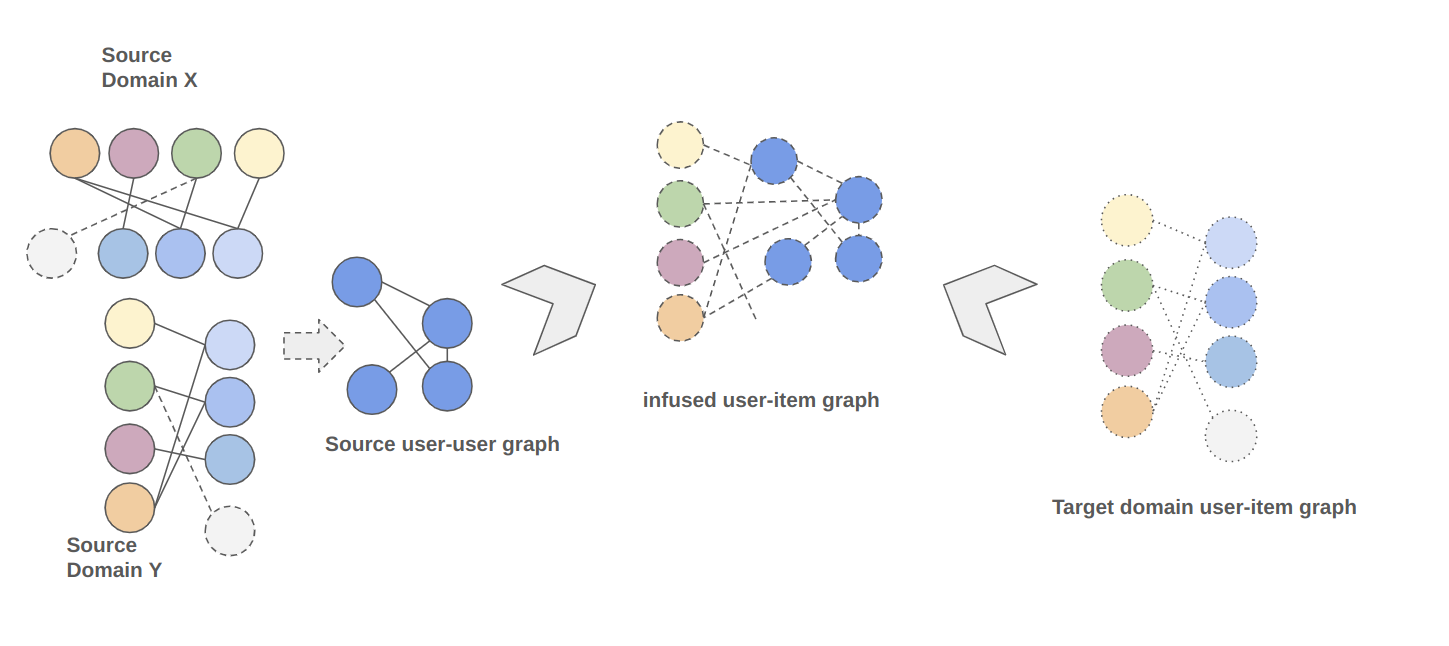
\includegraphics[width=1\textwidth]{figs/multi-graph-fusion.png}
    \caption{Illustration of the proposed method: The source domain data is first augment from user-item graph into a user-user graph. Then the augmented source user-user graph is then adapted into the target domain as a subgraph. finally the model is trained on the infused graph in a coherent way.}
    \label{fig:source-target-transfer}
\end{figure}

Leveraging information from other domains to enrich user and item representations in the target domain. However, some source domains frequently suffer from data sparsity issues themselves, introducing unwanted noise and reducing the effectiveness of the source data. Hence in our approach, we focuses on both the effectiveness and efficiency when transferring information from the source domain to the target domain. We first structure the bipartite graph for target domain, where the user and item nodes are connected by the interactions. Next, we leverage graph augmentation on source domain data, the augmented graph brings a number of benefits:

\begin{itemize}
    \item It can effectively improve graph density on shared nodes. (see more detailed comparison in section 4)
    \item Apply learnable edge regulation to adjust the edge weights based on the target domain data, which can effectively filter out the noises from the source domain data. e.g. reducing the impacts of highly connected nodes in the source domain, which may over weighted during the training process.
    \item user-user edges can be seamlessly integrated into the target domain graph, which can provide additional information for user representation learning.
\end{itemize}

We put adapt the augmented graph edges to the target domain by applying the edge regulation with a learnable weights.
The edge regulation is designed to adjust the edge weights based on the target domain data, which can effectively filter out the noises from the source domain data. e.g. reducing the impacts of highly connected nodes in the source domain, which may over weighted during the training process.
Finally, source and target domain data would be put through a GNN model to learn the user and item representations.
We use BPR as the optimization objective for training.
The user and item representations are learned jointly, thus, the information from the source domain is used to improve the target domain recommendation performance.
infuse target and source domains into a unified graph structure also improve the computational efficiency with less parameters to train, comparing to multi-graph approaches.

\subsection{Graph Construction for Target Domain}


\begin{figure}
    \centering
    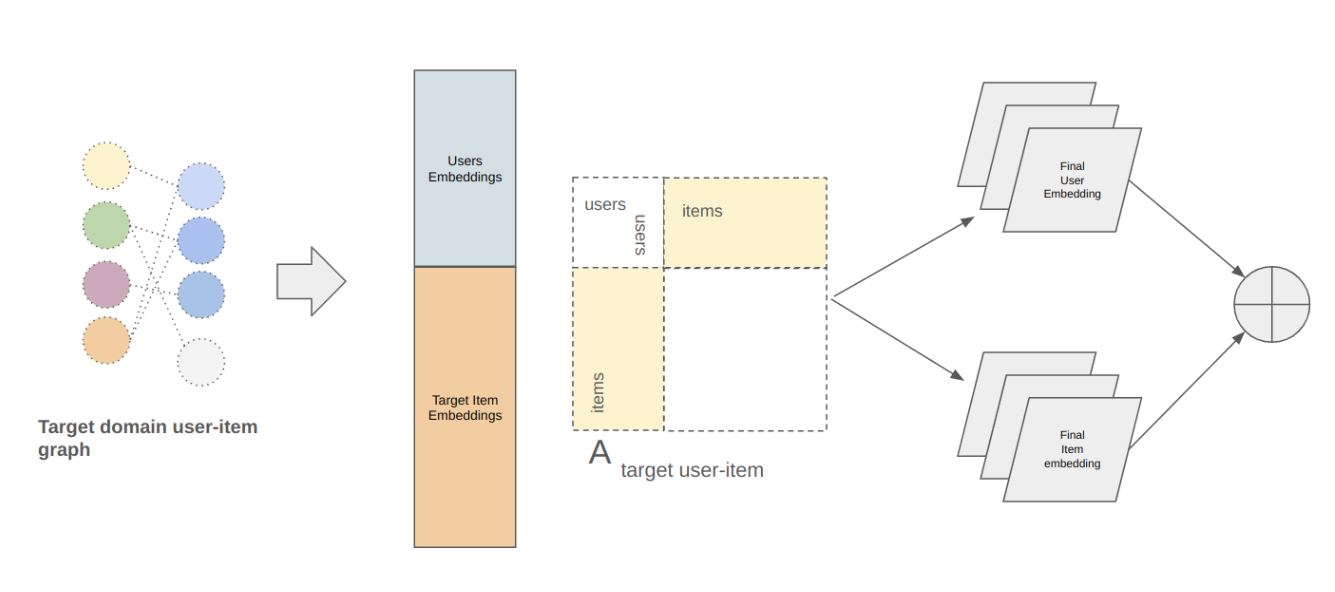
\includegraphics[width=1\textwidth]{figs/target-domain-graph.png}
    \caption{Illustration of LightGCN aggregator on target domain.}
    \label{fig:lightgcn}
\end{figure}


We define the domain user-item interactions as:
\begin{equation}
\centering
G = (V_{user/item}, E_{interaction})
\end{equation}

Where $V_{user/item}$ are the user and item nodes, and $E_{interaction}$ are the interactions between users and items in target Domain.

User and Item nodes presentation are learned using Graph Neural Network (GNN) model via nodes messaging and layer aggregation.

The basic GNN model aggregation can be abstract as:

\begin{equation}
\centering
e_u^{(k+1)} = AGG(e_u^(k),{e_i^(k), i \in N(u)})
\end{equation}

AGG can be different implementations of Aggregator such as GCN \cite{kipf2016semi, veličković2018graphattentionnetworks, hamilton2017inductive} are commonly used in GNN models.
The AGG function is the core of how message being propagated via nodes and its neighbors throughout the graph topology.
Those aggregators are designed to learn the node representation by using non-linear activation functions in feature transformation. Its effectiveness is proven in many classifier tasks.
However, when it comes to recommendation tasks, especially, when user interaction are only training dataset available.
The aggregator with nonlinearity functions commonly leads to over-smoothing issue, leads to poor performance and low variations in recommendation tasks \cite{Sharma2023ExperimentalHA}.

On the other hand, the aggregator, such as, LightGCN \cite{he2020lightgcn}, has proven results on improving the recommendation performance by adopting simple weighted sum aggregations, while reducing computation intensity at the same time.
During our experiments, we also found that LightGCN being more superior handling the over-smoothing issue, comparing to former mentioned aggregators.


In our approach, we construct the target domain graph as following.
we define a feature matrix for both user and item as E, while the adjacency matrix is defined as the user-item interaction matrix R=$R \in \mathbb{R}^{M \times N}$, where $M$ and $N$ are the user and item size.
hence the adjacency matrix can be presented as:

\begin{equation}
    E_{N+M} = \begin{pmatrix}
    E_{users} \\
    E_{items}
    \end{pmatrix},
    \quad
    A = \begin{pmatrix}
        0, & R_{N \times M} \\
        R^T_{M \times N}, & 0
        \end{pmatrix}
\end{equation}




hence, if we put the target domain through LightGCN aggregator:
\begin{equation}
E^{k+1} = (D^{-1/2} A D^{-1/2}) E^{k}
\end{equation}

We can get final user and item representation $e_{user}, e_{item}$ as:
\begin{equation}
    e_{user} = \sum_{l=0}^K \alpha_l e^{(l)}_{user};    \quad   e_{item} = \sum_{l=0}^K \alpha_l e^{(l)}_{item}
\end{equation}

where K is the number of layers in the GNN model, and $\alpha_l$ is the learnable weights for each layer.


\subsection{Source Domain Graph Augmentation}

\subsubsection{User-User Graph Augmentation}

\begin{figure}
    \centering
    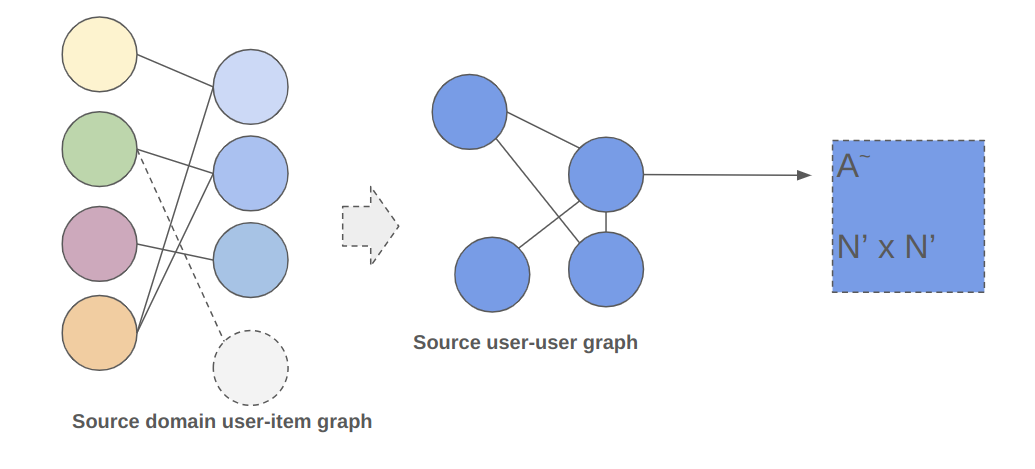
\includegraphics[width=1\textwidth]{figs/source-domain-graph.png}
    \caption{Illustration of the source domain user-user graph.}
    \label{fig:source-domain-graph}
\end{figure}

On the source domain side, we can derive the user-user or item-item graphs, based on common user/item interactions they share. (for simplicity, for the rest of the paper, we will use user-user graph as an example, the same logic can be applied to item-item graph as well.)

Say, the source domain has a user number of $N^{'}$ over lapping with the target domain $ N \cap N^{'}  >0 $. The source user-user graph presented as User Feature Embedding $E_{s}$, and the user-user interaction matrix $R_{s}$.:

\begin{equation}
    E_{s} = \begin{pmatrix}
    E_{N^{'}} \\
    \end{pmatrix},
    \quad
    A_{s} = \begin{pmatrix}
       R_{N^{'} \times N^{'}}
        \end{pmatrix}
\end{equation}

Apply degree normalization to the source user-user graph with weighted edges:

\begin{equation}
    A\tilde{~}_{s_ij} = \frac{ w_{s_ij}}{\sqrt{d_{s_i}} \sqrt{d_{s_j}}}
\end{equation}

The goal is remove the unuseable item nodes from the source. improving the density of the user-user graph, so the user similarity can be better learned and transferred to the target domain.


\subsubsection{Adapt Source Domain to Target Domain}

We adapt the source user-user adjacency matrix to the target domain user-item adjacency matrix.
Thus we get:

\begin{equation}
A_{infused} = \begin{pmatrix}
    0 + \begin{pmatrix}
        R_{N^{'} \times N^{'}}
        \end{pmatrix}, & R_{N \times M} \\
    R^T_{M \times N}, & 0

\end{pmatrix}
\end{equation}

Source User Feature Embedding $E_{s}$ will be shared with the target domain user feature embedding $E_{user}$, during training.

\begin{figure}
    \centering
    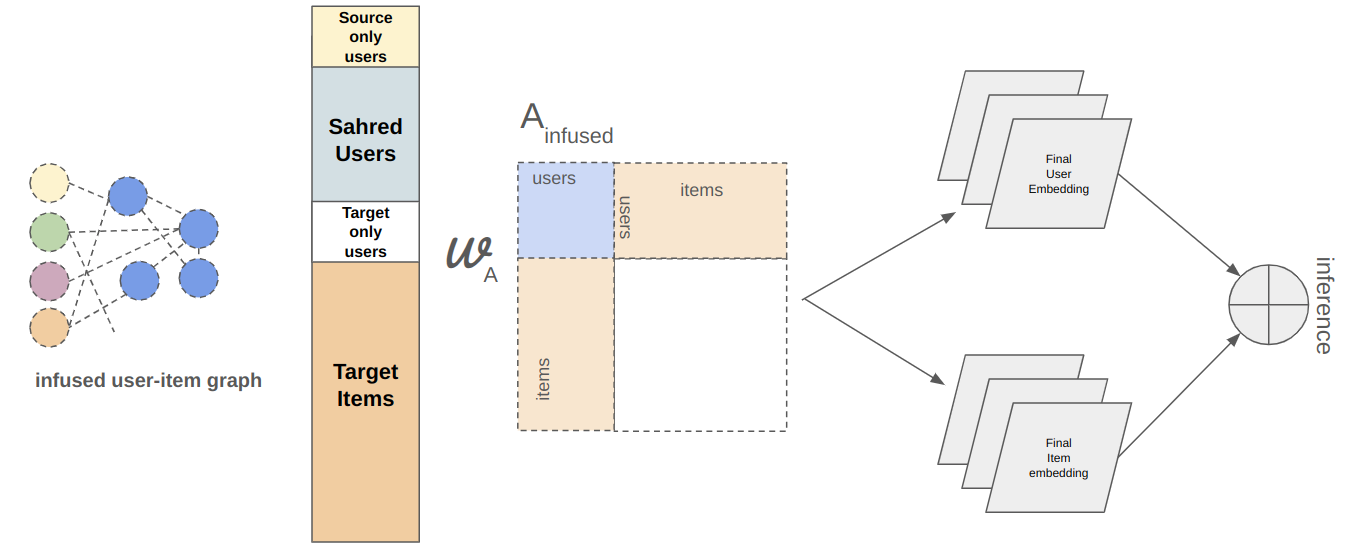
\includegraphics[width=1\textwidth]{figs/infused-domain-graph.png}
    \caption{Illustration of the source domain graph infusion to the target domain.}
    \label{fig:source-target-infusion}
\end{figure}

As we can see, during this process, fresh new users from the source, used to be out of target domain matrix, get introduced into the target domain from source. This enables the final model to make recommendation for those pure cold users, even no user-item interaction data is available in the target domain.
more details will be discussed in the experiment section.


\subsection{Model Training and Optimization}

\subsubsection{Source Domain Transfer Comparison}
Comparing to other source domain transfer methods, in general, we see the learning transfer is done via some form of dual or multi targets learning as model optimization objective.

A simplified loss function can be presented as:
\begin{equation}
    \begin{aligned}
        &\hat{y} = f_{target}(x_{target}) \\
        &\hat{y}^{'} = f_{source}(x_{source}) \\
        &L = L_{target} + L_{source} + \lambda L_{reg}
    \end{aligned}
\end{equation}

where $f_{target}$ and $f_{source}$ are the target and source domain models, $L_{target}$ and $L_{source}$ are the loss functions for target and source domain, and $L_{reg}$ is the regularization term.

CoNet \cite{Hu_2018} employs dual knowledge transfer across domains by introducing cross connections from one base network to another. Similarly, several other cross-domain recommender systems, such as PPNG \cite{zhao2019cross} and DTCDR \cite{DTCDR2019zhu}, adopt a similar approach with minor differences in their loss objectives, despite significant variations in their model architectures. In RecSys-DAN \cite{wang2019recsys}, transfer learning is achieved using a domain adversarial network.

A common aspect of these models above, are, all source embeddings are learned as part of the training process for knowledge transfer and domain alignment. Although these source domain embeddings are not used for the final recommendations, they still introduce additional parameters to train, increasing the model complexity.

\subsubsection{Simplified Taining Objective}

In our approach, we only use the source domain data to augment the target domain graph, hence no "waste" on the embedding learning for the model training. Thus, significantly reduces the model complexity and computational cost.

The trainable parameters in the model are the user and item embeddings, and the edge weights in the infused graph. the over lapped user between the source and target domain shares the same embeddings in the model.

We use Bayesian Probability Ranking as our optimization objective:

\begin{equation}
    L_{BPR} = -\sum\limits_{(u, i, j) \in E} \log \sigma(e_u \cdot e_i - e_u \cdot e_j)+  \lambda||E||^2
\end{equation}

Where $\sigma$ is the sigmoid function, $E$ is the set of user/item embeddings, $e$ is the embedding out put from the final layer. the $i$ and $j$ are the positive and negative samples for user $u$.
We use the L2 regularization, and the model is trained using Adam optimizer in mini batches.


%!TEX root = ./main.tex
\section{Experiments and Results}

First we will introduce the data set and experiment setup. Then we conduct experiments to evaluate the effectiveness through different scenarios and compare with other state-of-the-art base lines.


\subsection{Dataset and experiment setup}

We use amazon dataset for our experiments, which uses only user-item interactions as the input data.
more specifically, we picked 2 product categories BOOK and MUSIC.
between the 2 domains, we sampled 642 overlapping uniq users,  see Table \ref{tab:dataset} for more details.

\begin{table}[ht]
    \centering
    \begin{tabular}{|c|c|c|c|c|}
        \hline
        \textbf{Domain} & \textbf{Users} & \textbf{Items} & \textbf{Interactions} & \textbf{Density} \\ \hline
        BOOK (Target Domain)          & 642           & 3022         & 8857 & 0.00456               \\ \hline
        MUSIC (Source Domain)          & 642           & 3507         & 12434 & 0.00641             \\ \hline
    \end{tabular}
    \caption{Dataset statistics}
    \label{tab:dataset}
\end{table}

\subsubsection{Deriving a denser user-user graph from source domain}

\begin{table}[ht]
    \centering
    \begin{tabular}{|c|c|c|c|}
        \hline
        \textbf{Domain} & \textbf{Node number}  & \textbf{Edge number} & \textbf{Density} \\ \hline
        Source user-item       &  4149  & 8857 & 0.00456               \\ \hline
        Source user-user          & 642 & 46952 & \textbf{0.11391}             \\ \hline
    \end{tabular}
    \caption{Source domain user-user graph statistics}
    \label{tab:source-domain-user-user-graph}
\end{table}

We argument the source domain user-item graph to user-user graph.
The process, not only simplifies the source graph. the end results also significantly improves the density of the user-user graph.
while, it also effectively reduced the noises by discard source items nodes.
The fact that, the item feature is no use for the target domain recommendation. This also reduces the computational cost of the model.
see Table \ref{tab:source-domain-user-user-graph} for more details.



\subsection{Baseline comparison}

Fro the baseline comparison, we compare the following algorithms:

\begin{itemize}
    \item \textbf{BPR}: Bayesian Personalized Ranking
    \item \textbf{LightGCN}: Simplifying and Powering Graph Convolution Network for Recommendation
    \item \textbf{CoNet}: Deep Dual Transfer Cross Domain Recommendation
\end{itemize}

We use the following evaluation metrics to evaluate the performance of the recommendation algorithms:

\begin{itemize}
    \item \textbf{Precision@k} (P@k): the proportion of recommended items in the top-k that are relevant to the user.
    \item \textbf{Recall@k} (R@k): the proportion of relevant items in the top-k that are recommended to the user.
    \item \textbf{NDCG@k}: Normalized Discounted Cumulative Gain, which is a measure of ranking quality.
\end{itemize}


\subsection{Results}

We compare the performance of the proposed method with the baseline algorithms in terms of Precision@25, Recall@25, and NDCG@25. The results are shown in Table \ref{tab:results}.

\begin{table}[ht]
    \centering
    \begin{tabular}{|c|c|c|c|}
        \hline
        \textbf{Algorithm} & \textbf{Precision@25} & \textbf{Recall@25} & \textbf{NDCG@25} \\ \hline
        BPR          & 0.002852 & 0.017115 & 0.009939 \\ \hline
        LightGCN     & 0.005445 & 0.036747 & 0.024399 \\ \hline
        CoNet        & 0.003122 & 0.002123 & 0.016799 \\ \hline
        OURS         & \textbf{0.007714} & \textbf{0.048557} & \textbf{0.028301} \\ \hline
    \end{tabular}
    \caption{Results comparison}
    \label{tab:results}
\end{table}


\section{Conclusion and Future Work}
In this paper, we propose an infused graph framework for recommendation (CDGF). This framework offers a scalable and efficient solution suitable for large-scale recommendation systems. It supports various domain overlapping scenarios, including both partial and full overlapping data conditions on either common users or items. Additionally, it can handle multiple domains with different distributions and structures and can be easily extended to incorporate more domains.

We evaluated the effectiveness of the model on real-world datasets and demonstrated that it outperforms state-of-the-art methods in terms of recommendation accuracy, particularly effective in handling sparse data and cold-start scenarios, while using only implicit user-item interactions. Importantly, in an era where data privacy is a growing concern, our model achieves high-quality recommendations without relying on personally identifiable information (PII) or requiring complex data engineering efforts.

Future work will focus on extending the model to handle more complex scenarios, such as enhancing its inference ability to make transductive predictions and managing dynamic data changes within the graph architecture. These improvements will further enhance the model's accessibility and ultimately aid in the adoption of real-world recommender systems.


% \begin{appendices}

% \section{Section title of first appendix}\label{secA1}

% An appendix contains supplementary information that is not an essential part of the text itself but which may be helpful in providing a more comprehensive understanding of the research problem or it is information that is too cumbersome to be included in the body of the paper.

% \end{appendices}

%%===========================================================================================%%
%% If you are submitting to one of the Nature Portfolio journals, using the eJP submission   %%
%% system, please include the references within the manuscript file itself. You may do this  %%
%% by copying the reference list from your .bbl file, paste it into the main manuscript .tex %%
%% file, and delete the associated \verb+\bibliography+ commands.                            %%
%%===========================================================================================%%
\newpage
\bibliography{references}% common bib file
%% if required, the content of .bbl file can be included here once bbl is generated
%%\input sn-article.bbl

\end{document}
